%% this is necessary stuff to make the document compile:
\documentclass[reqno,11pt]{amsart}
\usepackage{amssymb, amsmath}
\usepackage{colordvi,verbatim,hyperref}
\usepackage{graphicx}
\usepackage{amsthm}

\usepackage[dvipsnames]{xcolor}
\usepackage{tikz}
\usetikzlibrary{positioning}
\usetikzlibrary{snakes}

%% this is for making margins the way I like them:
\headheight=8pt
\topmargin=0.375truein
\topmargin=-0.2truein
\textheight=9truein   \textwidth=6.3truein
\oddsidemargin=.1in \evensidemargin=.1in

%%this is to create new math commands. In other words, since I use theta^hat in equations a lot, I made a shorthand for it. So now instead of using $\hat\theta$ every time, I can just write $\thhat$. 
\newcommand{\Q}{{\mathbb{Q}}}
\newcommand{\N}{{\mathbb{N}}}
\newcommand{\R}{{\mathbb{R}}}
\newcommand{\rhs}{{\text{RHS}}}

\pagestyle{plain}


\date{\today}%7 Feb 2014}

\begin{document}
\title{An Analogy of Approximation Methods}
\author{Trenton Gerew}

\maketitle
	\begin{figure}[h!]
		\centering
		
		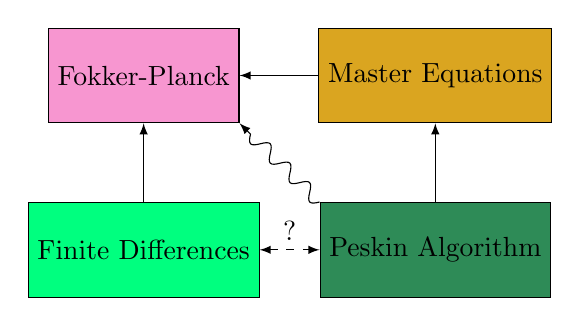
\begin{tikzpicture}
			% F-P
			\node [draw,
				fill=Rhodamine!50,
				minimum width=2cm,
				minimum height=1.2cm
				] (fp) at (0,0) {Fokker-Planck};
			
			% Master Equations
			\node [draw,
				fill=Goldenrod,
				minimum width=2cm,
				minimum height=1.2cm,
				right=1cm of fp
				] (me) {Master Equations};
				
			% Finite Differences
			\node [draw,
				fill=SpringGreen,
				minimum width=2cm,
				minimum height=1.2cm,
				below=1cm of fp
				] (fd) {Finite Differences};
				
			% Peskin Algorithm
			\node [draw,
				fill=SeaGreen,
				minimum width=2cm,
				minimum height=1.2cm,
				below=1cm of me
				] (pa) {Peskin Algorithm};
				
			% Arrows
			\draw[-latex] (me.west) -- (fp.east);
			\draw[-latex] (fd.north) -- (fp.south);
			\draw[-latex] (pa.north) -- (me.south);
			\draw[-latex,snake=coil,segment aspect=0] (pa.north west) -- (fp.south east);
			\draw[latex-latex,dashed] (fd.east) -- (pa.west)
				node[midway,above]{?};
		
		\end{tikzpicture}
		
		\caption{Approximation methods and their relationships to the Fokker-Planck equation. \label{fig:relationships}}
	\end{figure}

	The probability density $u (x,t)$ evolves according to the Fokker-Planck equation
	\begin{equation} \label{eq:f-p}
		\partial_t u (x,t) = \partial_x \left( u (x,t) \phi' (x) + \partial_x u (x,t) \right)
	\end{equation}
	where $\phi (x)$ is the potential energy.
	In one spatial dimension, \eqref{eq:f-p} is a simple convection-diffusion equation.
	
	First we will write an explicit finite difference scheme for \eqref{eq:f-p}.
	We assume we work on the closed domain $[0,1] \times [0,t_F]$.
	Note that we must use a finite time interval, but $t_F$ can be made as large as desired.
	We denote the spacings by $h$ and $s$ for space and time, respectively.
	Then the mesh points are
	\begin{equation*}
		(x_j = j h, t_n = n s), \ j = 0,1,2\dots,J, \ n = 0,1,2,\dots,
	\end{equation*}
	where $h = 1 / J$.
	We use the notation
	\begin{equation*}
		U_j^n \approx u (x_j,t_n).
	\end{equation*}
	to mean the approximations of the solution at the mesh points.
	
	The left side of \eqref{eq:f-p} is approximated using a forward difference for the time derivative:
	\begin{equation}
		\frac{U_j^{n+1} - U_j^n}{s} \approx \frac{\partial u (x_j,t_n)}{\partial t}.
	\end{equation}
	
	Next will we derive the approximation for the right side of \eqref{eq:f-p}.
	We first approximate $\phi'(x)$ as a constant at any space step $j$ with the forward difference
	\begin{equation}
		\frac{\phi(x_{j+1}) - \phi(x_j)}{h} \approx \phi'(x_j).
	\end{equation}
	Therefore, the RHS can be written as
	\begin{equation*}
		\rhs = u_x \phi' + u_{xx}.
	\end{equation*}
	Now using a forward difference and a centered second difference to approximate $u_x$ and $u_{xx}$ respectively, we have
	\begin{equation}
		\left( \frac{\phi_{j+1} - \phi_j}{h} \right) \left( \frac{U_{j+1}^n - U_j^n}{h} \right) + \frac{U_{j+1}^n - 2 U_j^n + U_{j-1}^n}{h^2} \approx \partial_x \left( u (x_j,t_n) \phi' (x_j) + \partial_x u (x_j,t_n) \right).
	\end{equation}
	Thus, the explicit scheme is
	\begin{equation}
		U_j^{n+1} = U_j^n + \frac{s}{h^2} \left( U_{j+1}^n (1 + \Delta \phi_j) - U_j^n (2 + \Delta \phi_j) + U_{j+1}^n \right)
	\end{equation}
	where $\Delta \phi_j = \phi(x_{j+1}) - \phi(x_j)$.
\end{document}